\documentclass[12pt]{article}

\usepackage{fullpage}
\usepackage{graphicx, rotating, booktabs} 
\usepackage{times} 
\usepackage{natbib} 
\usepackage{indentfirst} 
\usepackage{setspace}
\usepackage{grffile} 
\usepackage{hyperref}
\usepackage{adjustbox}
\usepackage{amsmath}
\usepackage{siunitx}
\setcitestyle{aysep{}}


\singlespace
\title{\textbf{The Sources of Alliance Treaty Depth}}
\author{Joshua Alley\footnote{Graduate Student,
Department of Political Science, Texas A\&M University.}}
\date{}

\bibliographystyle{apsr}

\begin{document}

\maketitle 

\doublespace 

\begin{abstract}
Why do states form deep alliances? 
Deep treaties add defense coordination and cooperation to promises of military support.
I argue that alliances between democracies are especially likely to include high treaty depth. 
In these alliances, members use treaty depth as a substitute for commitments of unconditional military support.
Using several statistical models, I show that decisions to include depth and unconditional military support in alliance treaties are correlated.
Moreover, I find that as the average democracy of alliance members at the time of formation increases, treaty depth increases, but the probability the treaty offers unconditional military support decreases. 
Thus, democracies do not uniformly offer limited commitments, but instead they substitute different sources of treaty depth. 
The argument and findings have important implications for our understanding of the process and consequences of alliance treaty design. 
\end{abstract}


\newpage 


\section{Introduction}


% Start with hook: maybe a story of a deep and shallow alliance 
Why do states make deep alliance treaties? 
While some alliance treaties include only a promise of military support, others supplement military support with commitments of extensive defense cooperation. 
To give a well-known example, the formal NATO treaty commits to setting up a formal international organization to govern the alliance. 


Depth is a common part of alliances and varies greatly across treaties. 
At least half of all ATOP alliances with offensive or defense obligations have at least one source of treaty depth.
Moreover, the prevalence of deep alliances increased after 1945. 


% Deep alliances matter: affect milex, maybe credibility 
Adding formal treaty depth to an alliance has important consequences. 
Deep alliances encourage  non-major power members to reduce military spending because treaty depth increases alliance credibility.  
On the other hand, participation in shallow alliances increases military spending because partners can use the threat of abandonment as bargaining leverage. 
\autoref{fig:depth-motive} shows this relationship. 
The issue of military spending shows treaty depth affects alliance politics by shaping treaty credibility and the distribution of military spending burdens among members. 


\begin{figure}[hbtp]
\centering
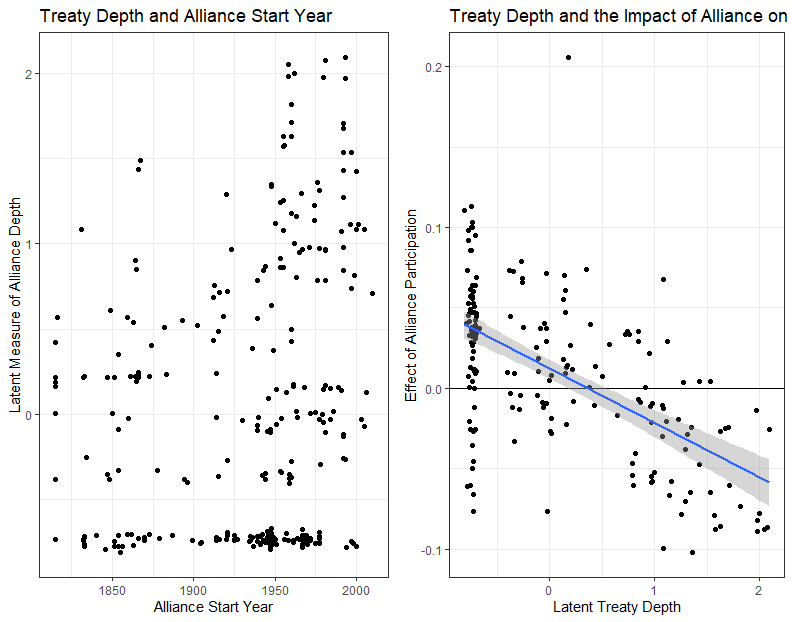
\includegraphics[width=0.95\textwidth]{../figures/depth-motive.png}
\caption{This scatter plot shows that the impact of alliance participation on non-major power military spending falls as treaty depth increases. I created this measure of depth measure using a latent variable model. Values around -0.8 are alliances with no depth, so larger values imply the treaty has at least some depth.}
\label{fig:depth-motive}
\end{figure}


% Describe question and contribution of the paper
Despite the consequences of alliance treaty depth, we know little about when states add depth to their alliances.\footnote{\citet{Mattes2012} examines a few possible causes of military institutionalization.}
In this paper, I explain when states form deep alliances.
I argue that alliance member characteristics shape conditions on military support in the treaty, which then affect treaty depth. 
Alliance negotiations center on whether prospective members will offer military support and conditions on that support \citep{Poast2019a}. 
When alliance members are unwilling to offer unconditional military support, they can use depth as a substitute source of reliability.%\footnote{Depth could also complement promises of unconditional military support in alliances among autocracies.}


Because democracies tend to offer alliances with conditional obligations \citep{Mattes2012, Chibaetal2015}, they also increase treaty depth. 
Democracies make conditional promises because leaders fear audience costs of violation, and limited commitments are harder to violate.
At the same time, these limited alliances can increase other alliance partners' fear of abandonment. 
Therefore, democracies can use costly provisions in deep alliances as an alternative source of credibility.   


I test this argument with a series of statistical models and an illustrative case study.
The statistical models employ multiple equations to approximate the alliance negotiation process as well as the correlation between depth and unconditional military support. 
The case studies check the theoretical process and statistical results \citep{SeawrightGerring2008, Seawright2016}. 
I find consistent evidence that as allied democracy at the time of alliance formation increases, treaty depth increases and unconditional military support is less likely. 


% Para on implications: sources of credibility and reassurance are connected
My argument and findings have important consequences for research on alliance treaty design. 
Existing scholarship considers individual parts of treaty design in isolation \citep{Benson2012, Mattes2012, Chibaetal2015}. 
My argument shows that sources of credibility in alliance treaty design are connected. 
Theorizing about and modeling different alliance characteristics in isolation may generate misleading conclusions. 
Previous estimates of the connection between democracy and treaty depth produced null findings, in large part because previous models do not consider the association between depth and conditions on military support. 


% Paragraph on the importance of democracy in alliance pol
This paper adds to knowledge of how democracy and domestic politics shape alliance politics. 
Scholars have long acknowledged that democracy and alliances are connected \citep{LaiReiter2000, GiblerWolford2006, Warren2016, McManusYarhi-Milo2017}. 
Democratic commitments are often seen as more credible due to audience costs \citep{DigiuseppePoast2016}. 
My argument suggests that although democracies do screen the scope of their commitments carefully, they form deeper alliances on other dimensions.  


% roadmap for the paper 
The paper proceeds as follows. 
In the next section, I lay out the argument and hypothesis. 
Then I describe the data and research design 


\section{Argument}


In this argument, I start by establishing a definition of treaty depth. 
Then, I show that treaty depth is understudied with a brief review of existing work on alliance treaty design. 
After that, I describe a general model of the process of alliance treaty negotiations. 
Finally, I describe how alliance negotiations between non-major powers tend to lead to higher treaty depth. 


% define alliance treaty depth
Alliance depth is the extent of defense cooperation formalized in the treaty. 
Deep alliances require additional military policy coordination and cooperation. 
While shallow alliances stipulate more arms-length ties between members, deep treaties lead to closer cooperation through intermediate commitments that fall between no alliance active and military intervention. 
Defense cooperation in a deep alliance takes many forms. 
Allies can form an integrated military command, provide military aid, commit to a common defense policy, provide basing rights, set up an international organization or undertake companion military agreements. 


% note that I'm the first one to address this question: lit review. 
Depth is therefore an important part of alliance treaty design.
In general, alliances can be thought of as self-enforcing contracts or institutions \citep{Leedsetal2002, Morrow2000}.
Given external threats in an anarchic international system, states form alliances to aggregate military capability and secure their foreign policy interests \citep{Altfield1984, Smith1995, Snyder1997, FordhamPoast2014}. 


Potential alliance members can design a wide range of treaties \citep{Leedsetal2000, Leedsetal2002, Benson2012, BensonClinton2016}. 
Design considerations shape the costs and benefits of treaty participation. 
Beyond the benefits of potential military support and deterrence, alliances also clarify international alignments \citep{Snyder1990} and support economic ties \citep{Gowa1995, Li2003, Long2003, Fordham2010, WolfordKim2017}. 
The costs of alliances include lost foreign policy autonomy \citep{Altfield1984, Morrow2000, Johnson2015}, as well as the risk of opportunistic behavior. 
Potential opportunism in alliances includes abandonment, or the failure of alliance members to honor their commitments \citep{BerkemeierFuhrmann2018}, entrapment in unwanted conflicts \citep{Snyder1984}, and free-riding \citep{Morrow2000}.   


% Depth is understudied
Treaty design can address reliability concerns and the risk of entrapment, but the process of alliance treaty design is understudied \citep{Poast2019a}. 
\citet{Mattes2012} offered an early study of alliance treaty design by using symmetry of capability and history of violation to explain conditions on military support, issue linkages, and military institutionalization in bilateral alliances. 
She argues that all three design considerations increase treaty reliability and finds mixed evidence.  
While checking the validity of their latent measure of treaty depth, \citet{BensonClinton2016} find that foreign policy disagreements, major power involvement and treaty scope are all positively correlated with depth. 
Their latent measure of scope is based on the type of military support offered and conditions on that support. 


We have a better sense of when states offer conditional military support. 
\citet{Benson2012} shows that foreign policy disagreements and revisionist protege states increase the likelihood of limited military support commitments.
\citep{Chibaetal2015} added to to existing work on limited obligations by showing that democracies are more likely to form alliances with conditional military support or consultation. 
Other work by \citet{Poast2012, Poast2013} establishes that states often use issue linkages to facilitate alliance formation. 


None of these works link treaty scope and depth.  
\citet{Mattes2012} studies military institutionalization and conditionality as separate sources of reliability. 
Her argument and research design treat depth and institutionalization as independent.
Though \citet{BensonClinton2016} use scope to predict depth and depth to predict scope, they do not consider the correlation between the two processes. 
Perhaps as a result of these theoretical and empirical choices, both works on treaty depth finds no association between the democracy of alliance members and military institutionalization. 
Because states can use different foreign policy instruments as substitutes or complements \citep{Starr2000, MorganPalmer2000}, treaty depth and conditions on military support are probably related. 
My argument builds on existing scholarship by placing depth and conditions on military support in a unified theoretical and empirical framework. 
I now describe the general process of the argument. 


\subsection{Alliance Negotiations and Obligations}


% process of alliance negotiations: once agreed on military support, need to bolster. 
Alliance treaty design is the result of negotiations between members \citep{Poast2019a}.  
Negotiations must determine conditions or limitation on military support and treaty depth.\footnote{The alliance formation stage is something I will need to model in a later robustness check.}
Both stages address the benefits and costs of alliance participation, along with the risk of opportunism, albeit in different ways. 


% Part 1: Establish military support and conditions on that support
Establishing if and when military support will be offered is the essential task for potential alliance partners. 
Promises of military intervention are the core of alliances. 
To form an alliance, the members must have sufficient overlap in foreign policy interests \citep{Morrow1991, Smith1995, FordhamPoast2014}, especially their proposed war plans \citep{Poast2019a}.  


Promises of military support in an alliance vary widely, however. 
The extent of shared foreign policy interests shapes whether alliance members offer unconditional or conditional military support.
Many alliances limit promises of intervention to particular regions, conflicts, or instances of non-provocation \citep{Leedsetal2000}. 
For example, if alliance members fear entrapment in unwanted conflicts, they will only offer military support in specific circumstances \citep{Kim2011, Benson2012}.\footnote{Such deliberate design of alliances means clear instances of entrapment are rare \citep{Kim2011, Beckley2015}.} 
Conditional treaties reflect less overlap in foreign policy interests. 


Offering unconditional military support is thus a strong signal of shared foreign policy interests. 
Attaching no conditions to a potential intervention means alliance members hazard the reputational \citep{Gibler2008, Crescenzietal2012} and audience \citep{Fearon1997} costs of treaty violation as they can be pulled into many conflicts. 
Accepting these potential costs implies that conflict participation is acceptable--- there is less fear of entrapment and many shared foreign policy interests. 
As a result, unconditional alliances are a key source of credibility. 


% Part 2: depth
To complement conditions on military support, alliance partners also negotiate over how to reinforce those promises and put them into action. 
This component of alliance negotiations determines the depth of the treaty. 
Depth shapes the perceived reliability of the treaty by providing opportunities for states to fulfill treaty obligations in peacetime. 
Implementing deep treaty provisions can also enhance joint war-fighting. 


Treaty depth depends on member characteristics and conditions on promises of military support from the first stage of the negotiations.
Potential conditions on military support also depend on treaty depth. 
Therefore, there is a reciprocal relationship between conditions on military support and treaty depth. 
States can form alliances with any combination of depth and conditions. 


Though depth and conditions on military support are related, they are not equivalent. 
Both affect alliance reliability, but they vary in how their costs are expressed. 
Conditions on military support do not change absent treaty renegotiation, and their potential costs remain hypothetical unless the alliance is invoked.  
But time-inconsistency problems due to changing foreign policy interests are a major threat to alliance fulfillment \citep{LeedsSavun2007}. 
Although unconditional promises of military support are more credible, they are also vulnerable to changing foreign policy interests. 
Under a deep alliance treaty, members can use implementation of defense cooperation and policy coordination to assess allied reliability. 
Observing that alliance members adhere to peacetime promises indicates they will also honor promises of military support. 
Therefore, depth can increase the perceived reliability of conditional or unconditional military support. 


This connection between depth and conditions on military support means that understanding how alliance member characteristics affect alliance treaty design must account for both sources of credibility.  
Depth and conditionality are distinct sources of reliability, but they have a common function. 
As I detail below, democracies are more likely to design alliances with conditional military support. 
As a result of this decision, democracies use greater treaty depth to address reliability concerns from these limited commitments.  
Democratic alliances therefore offer limited military support and high depth. 


\subsection{Alliances between Democracies}


% Start with a well-established result: democracy and conditional obligations
There is already ample evidence that democracies often prefer conditional military support. 
\citet{Mattes2012} and \citet{Chibaetal2015} both show that democracies are more likely to design conditional alliances. 
They attribute this tendency to higher audience costs in democracies. 
Because democratic leaders face substantial audience costs from violating their international commitments, leaders design more limited commitments that are easier to fulfill. 
Based on this logic, even after accounting for the correlation between depth and scope, increasing the average democracy of alliance members at the time of formation should reduce the probability of unconditional military support.


\begin{quote}
\textsc{Unconditional Military Support Hypothesis: As the average democracy of alliance members at the time of formation increases, the probability that the alliance will include unconditional military support will decrease.}
\end{quote} 


% Move to treaty depth: look at it from a reliability perspective
Limiting alliance commitments through conditional military support reduces audience costs because it is easier for democratic leaders to backtrack on military support. 
Under a conditional alliance, states are not automatically obligated to intervene. 
As a result, it is possible for leaders to either claim that the conditions for intervention were not met, or that new information obviates the alliance commitment \citep{LevenduskyHorowitz2012}. 


Because allied states understand these limits on conditional alliances, conditional promises will increase reliability concerns. 
Knowing that allies have given themselves an out will increase the fear of abandonment. 
Therefore, democracies may need to find other ways to indicate their commitments are credible. 


Democracies can use depth as a substitute for unconditional military support. 
By including peacetime costs in a deep alliance, democratic states provide a different signal of reliability. 
Providing regular access to military aid, bases, or policy coordination indicates that alliance members are committed to the treaty. 
This increases allied confidence that democracies will honor their treaty obligations, even if the conditions on those obligations are limited. 
Willingness to form a deep alliance makes conditions on military support tolerable. 


Moreover, depth is a flexible way for democratic states to increase the perceived reliability of their alliances. 
Rather than make a fixed commitment of unconditional military support, democracies can shift their commitment to an alliance if electoral politics requires it.
For example, democratic leaders could reduce military aid to an ally if their constituents prefer a more limited foreign policy.  
Therefore, leaders are less constrained by the alliance choices of previous leaders, as they have some freedom to change how many peacetime costs they bear. 


Depth has more flexibility for democratic leaders because there are lower audience costs for not fulfilling peacetime promises. 
While military intervention is costly and highly public, the day to day aspects of alliance management are less salient for the public. 
Elite dissension about changes in commitment to a deep alliance is unlikely to translate into meaningful public opposition and electoral concerns. 


% express the key hypotheses
As a result of their proclivity to offer conditional military support and the lower audience costs of treaty depth, democracies will be more likely to design deep alliance treaties. 
Put differently, as the average democracy of alliance members at the time of treaty formation increases, treaty depth should increase. 


\begin{quote}
\textsc{Treaty Depth Hypothesis: As the average democracy of alliance members at the time of formation increases, the depth of an alliance treaty will increase.}
\end{quote} 


% brief case illustration 
Many democratic alliances combine conditional military support and high treaty depth. 
Consider a 1960 defense pact between the United States and Japan (ATOPID 3375).
This alliance updated a 1951 defense treaty and included conditional obligations of military support. 
Promises of intervention are conditional on whether the fighting is taking place in East Asia. 
Moreover, the signatories promised action ``to meet the common danger'' if a member is attacked, which is not an explicit promise of military support. 
These kinds of limited promises are common in US alliances. 
The United States and Japan simultaneously formed a Security Consultative committee and permitted US troop bases in Japan, which are both sources of treaty depth. 


There is an important caveat to this argument--- I am interested in institutional design, not implementation.
Alliance treaty depth is not always implemented fully, as treaty aspirations are not fully realized, or work poorly. 
To give one example, several deep Arab alliances never realized their full intention due to internal political divisions.  


Based on the argument and the case example, I expect that alliance negotiations between non-major powers will produce deeper alliance treaties. 
The main mechanism behind this relationship is unconditional military support, because treaty depth supports unconditional obligations. 
Non-major powers also use depth to maximize their limited military capabilities. 
In the next section, I describe how I will test this claim about the association between non-major power membership and treaty depth. 




\section{Research Design}


My argument claims that the processes behind deep treaties and conditions on military support are related. 
Therefore, the research design uses multiple equations with correlated errors to assess how democracy affects the inclusion of unconditional military support and depth in alliance treaties.
I start by describing the key variables in the analysis. 
Then I provide more detail on the estimation strategy. 


% start with data
To examine my prediction that democracies tend to produce conditional alliances with substantial depth, I employ data on alliance treaty design from the Alliance Treaty Obligations and Provisions dataset \citep{Leedsetal2002}. 
I focus on 289 alliances with either offensive or defensive obligations, which is the set of treaties with military support. 
All results in the paper use these 289 alliances as the sample, and I will assess robustness to adjusting for non-random selection into alliances in the appendix. 


Using the ATOP data, I used a semiparametric mixed factor analysis to measure alliance treaty depth \citep{Murrayetal2013}.\footnote{See \textbf{\href{https://github.com/joshuaalley/arms-allies/blob/master/manuscript/arms-allies-paper.pdf}{this paper}} for more details on the measure.}
This measure of depth is weighted combination of ATOP's defense policy coordination, military aid, integrated military command, formal organization, companion military agreement, specific contribution, and bases variables. 
Each of these individual indicators increases alliance treaty depth, but defense policy coordination and an integrated command have the largest positive association, as shown in the top panel of \autoref{fig:loadings-measure}. 


\begin{figure}[hbtp]
\centering
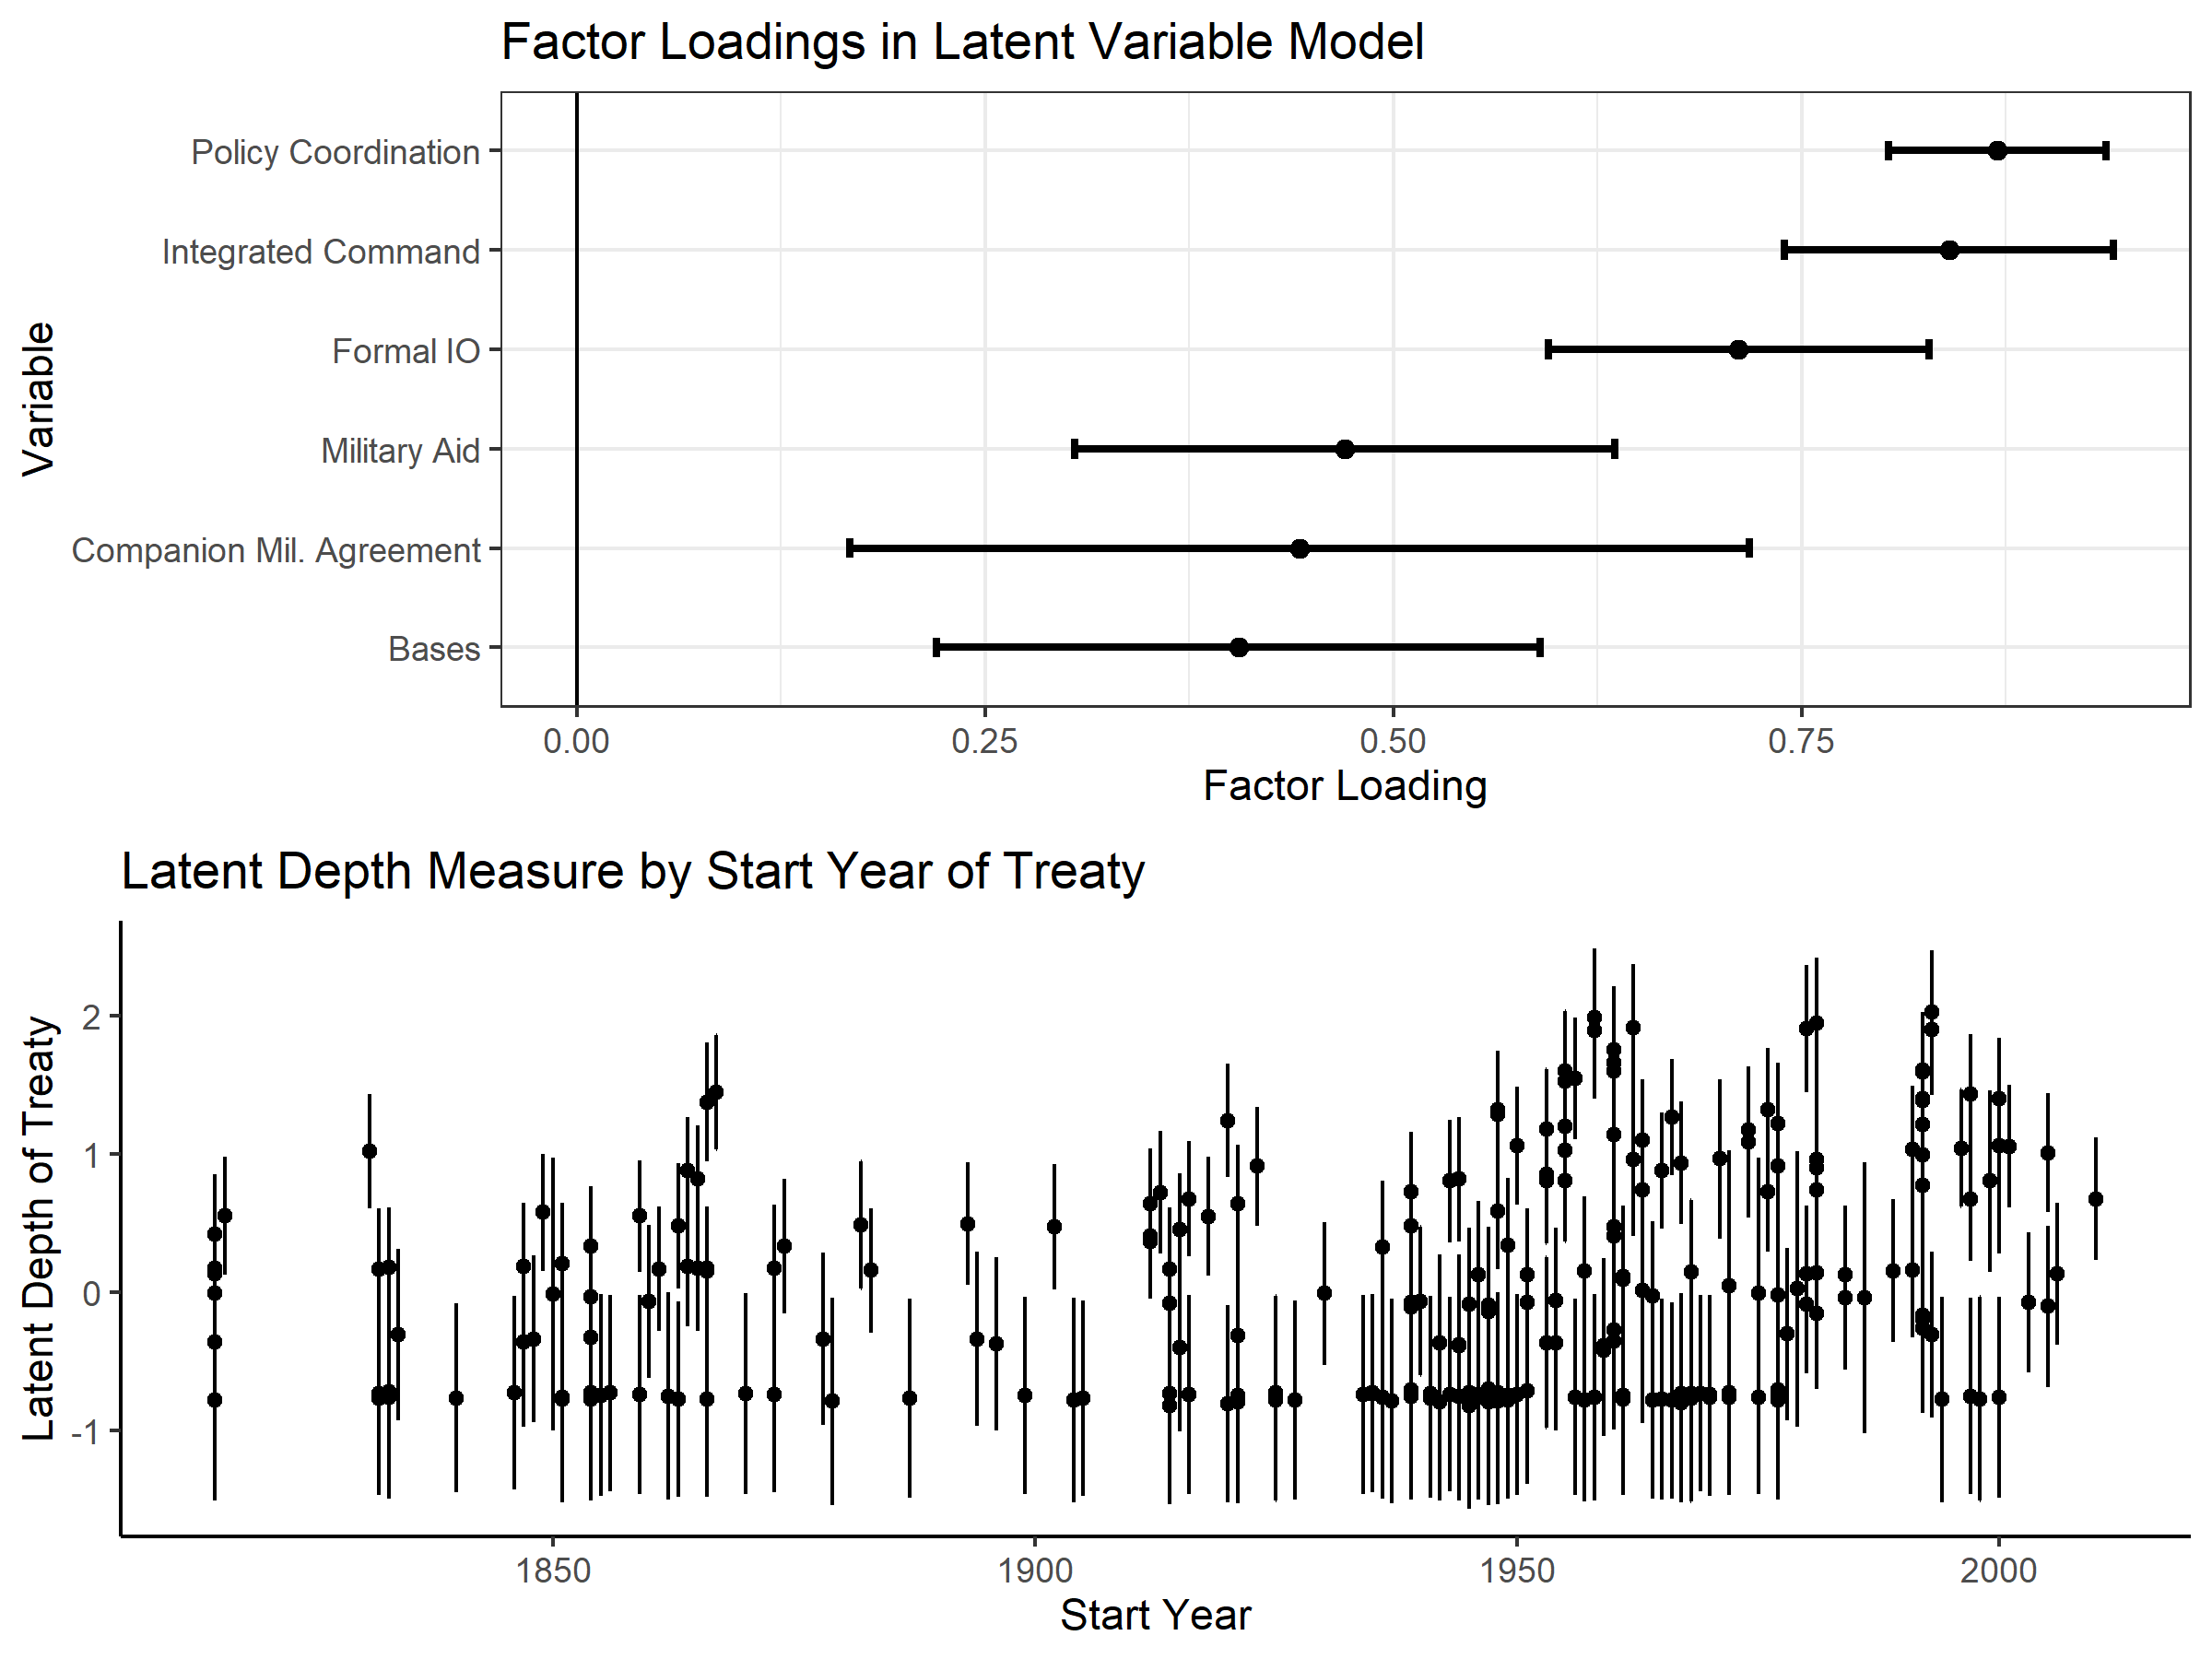
\includegraphics[width=0.95\textwidth]{../figures/loadings-measure.png}
\caption{Factor Loadings and posterior distributions of latent alliance treaty depth measure.}
\label{fig:loadings-measure}
\end{figure}


Based on these factor loadings, the measurement model predicts the likely value of treaty depth. 
The distribution of depth is summarized by the bottom panel of \autoref{fig:loadings-measure}. 
There is substantial variation in alliance treaty depth. 
Around half of all formal alliance treaties have an least some depth, and once states add some depth, there is a wide range of how much they include.


I measure alliance treaty depth in three ways.
First, I take the posterior mean of the latent depth posterior for each alliance. 
I also fit a statistical model that accounts for posterior uncertainty in the latent measure. 
Last, I measure alliance treaty depth with a dummy indicator of whether the alliance has greater than median depth. 
Results from these three measures are very similar. 


The second outcome variable is a dummy indicator of unconditional military support. 
Using ATOP's information on whether defensive or offensive promises are conditional on specific locations, adversaries, or non-provocation, I set this variable equal to one if the treaty placed no conditions on military support.
123 of 289 alliances in the data have unconditional military support. 

The key independent variable is the average democracy of alliance members at the time of treaty formation. 
I use the POLITY measure of regime type to measure democracy. 
I also consider a ``strongest link'' measure, which is the maximum democracy value at the time of formation.


% Justify this choice compared to a joint democracy dummy
An alternative measure of democracy is a dummy variable which is equal to one if both alliance members have a polity score greater than 5. 
I prefer the average and maximum polity score measures because they translate better to multilateral alliances. 
Moreover, democracy in one member will impact alliance treaties with less democratic partners, and a joint democracy variable would not capture that effect. 


Hypothesis 1 expects that as average democracy in an alliance increases, the probability of unconditional military support in the treaty decreases.
Hypothesis 2 predicts a positive association between democracy and treaty depth. 
I now describe how I examine these predictions. 


\subsection{Estimation Strategy}


Because there is feedback between unconditional military support and treaty depth, I specify a statistical model with two equations and correlated errors. 
One model predicts the probability unconditional military support, and the other predicts treaty depth.
Unconditional military support is included as a predictor of depth, and depth also predicts unconditional military support.  
I also corroborate correlations from the statistical models, through case study evidence that shows how the sequence of alliance negotiations matches my theoretical argument and the empirical results. 


To model unconditional military support, I fit a binomial model with logistic link function. 
The average democracy dummy is the key independent variable, and I also control for a range of other factors.
All of these variables could be correlated with unconditional military support and non-major power membership. 
Key controls include a dummy for asymmetric capability \citep{Mattes2012} and the average threat among alliance members at the time of treaty formation \citep{LeedsSavun2007}. 
I also control for foreign policy similarity \citep{Benson2012} using the minimum value of Cohen's $\kappa$ in the alliance \citep{Hage2011}.
Using the ATOP data \citep{Leedsetal2002}, I control for asymmetric treaty obligations, the number of alliance members, whether any of the members were at war and the year of treaty formation. 
To capture the role of issue linkages in facilitating alliance agreements \citep{Poast2012, Poast2013}, I also include a dummy indicator of whether the alliance addressed economic issues.  
Last, I include a count of foreign policy concessions in the treaty, because concessions can facilitate alliance negotiations \citep{Johnson2015}. 


The model of treaty depth retains all of the above control variables and the average democracy variable. 
All these variables could conceivably alter the need for additional reliability from treaty depth. 
I then add the unconditional military support dummy to this specification. 
Modeling depth is more complicated because the latent measure is a extremely skewed.
To facilitate model fitting, I transformed latent depth by transforming the variable to range between zero and one, then used a beta distribution for outcome.\footnote{I also considered log-logistic, Dagum and inverse Gaussian distributions for the outcome, but the beta model gave the best predictions.}
The flexibility of the beta distribution helps predict mean latent depth and facilitates fitting models that account for uncertainty in the latent measure, which I describe in more detail below. 
As an alternative measure of the outcome, I also fit a model with a dummy variable indicating whether the latent depth of the treaty was greater than the median depth value. 


I fit the mediator and outcome models simultaneously using generalized joint regression modeling (GJRM) \citep{Braumoelleretal2018}.
GJRM uses copulas to model correlations in the error terms of multiple equation models, which makes it more flexible than parametric models and facilitates causal inference. 
Modeling any unobserved correlation between depth and unconditional military support facilitates accurate inferences about democracy and other covariates. 
Copulas are distributions over functions, and model fit can express both the symmetry and direction of the dependence between the outcomes. 
While the substitution argument suggests a symmetric copula will best capture the dependence between depth and conditionality, I fit models with all copulas, and selected the best-fitting model using AIC, conditional on that estimator having converged.\footnote{GJRM is estimated with maximum likelihood, and diagnostics for the gradient as well as the information matrix suggest that the GJRM models converged.} 
The symmetric T copula, provides the best model fit. 


GJRM also facilitates checking for non-linear relationships by allowing smoothed terms. 
I estimated smoothed terms for democracy, mean threat and the start year of the alliance to capture potential non-linear relationships.\footnote{Fitting models with other continuous terms smoothed returned effective degrees of freedom = 1 for foreign policy similarity, which suggests a linear fit is equivalent. As the the results will show, the smoothed term for democracy is highly linear.}  
In the next section, I summarize the results of the analysis. 



\section{Results}


My findings are consistent with the claim that increasing democracy in an alliance leads to treaties with conditional support and greater depth. 
In this section, I first offer some descriptive statistics that are consistent with my claim, before turning to inferences from full models. 


First, unconditional alliances tend to have lower average democracy values. 
The average of democracy among alliances with unconditional military support is -3.7. 
Conversely, average polity score in alliances with conditional obligations is -1.9.\footnote{Based on a t-test, the difference between these values is statistically significant.} 
There is also a slight positive correlation between average alliance democracy at the time of formation and treaty depth. 

% plot 
\autoref{fig:democ-combo} shows the mix of unconditional military support and high treaty depth in alliance design as democracy increases. 
Triangular points mark unconditional military support. 
At high levels of democracy, there are more conditional treaties, and most alliances have some depth. 


\begin{figure}[hbtp]
\centering
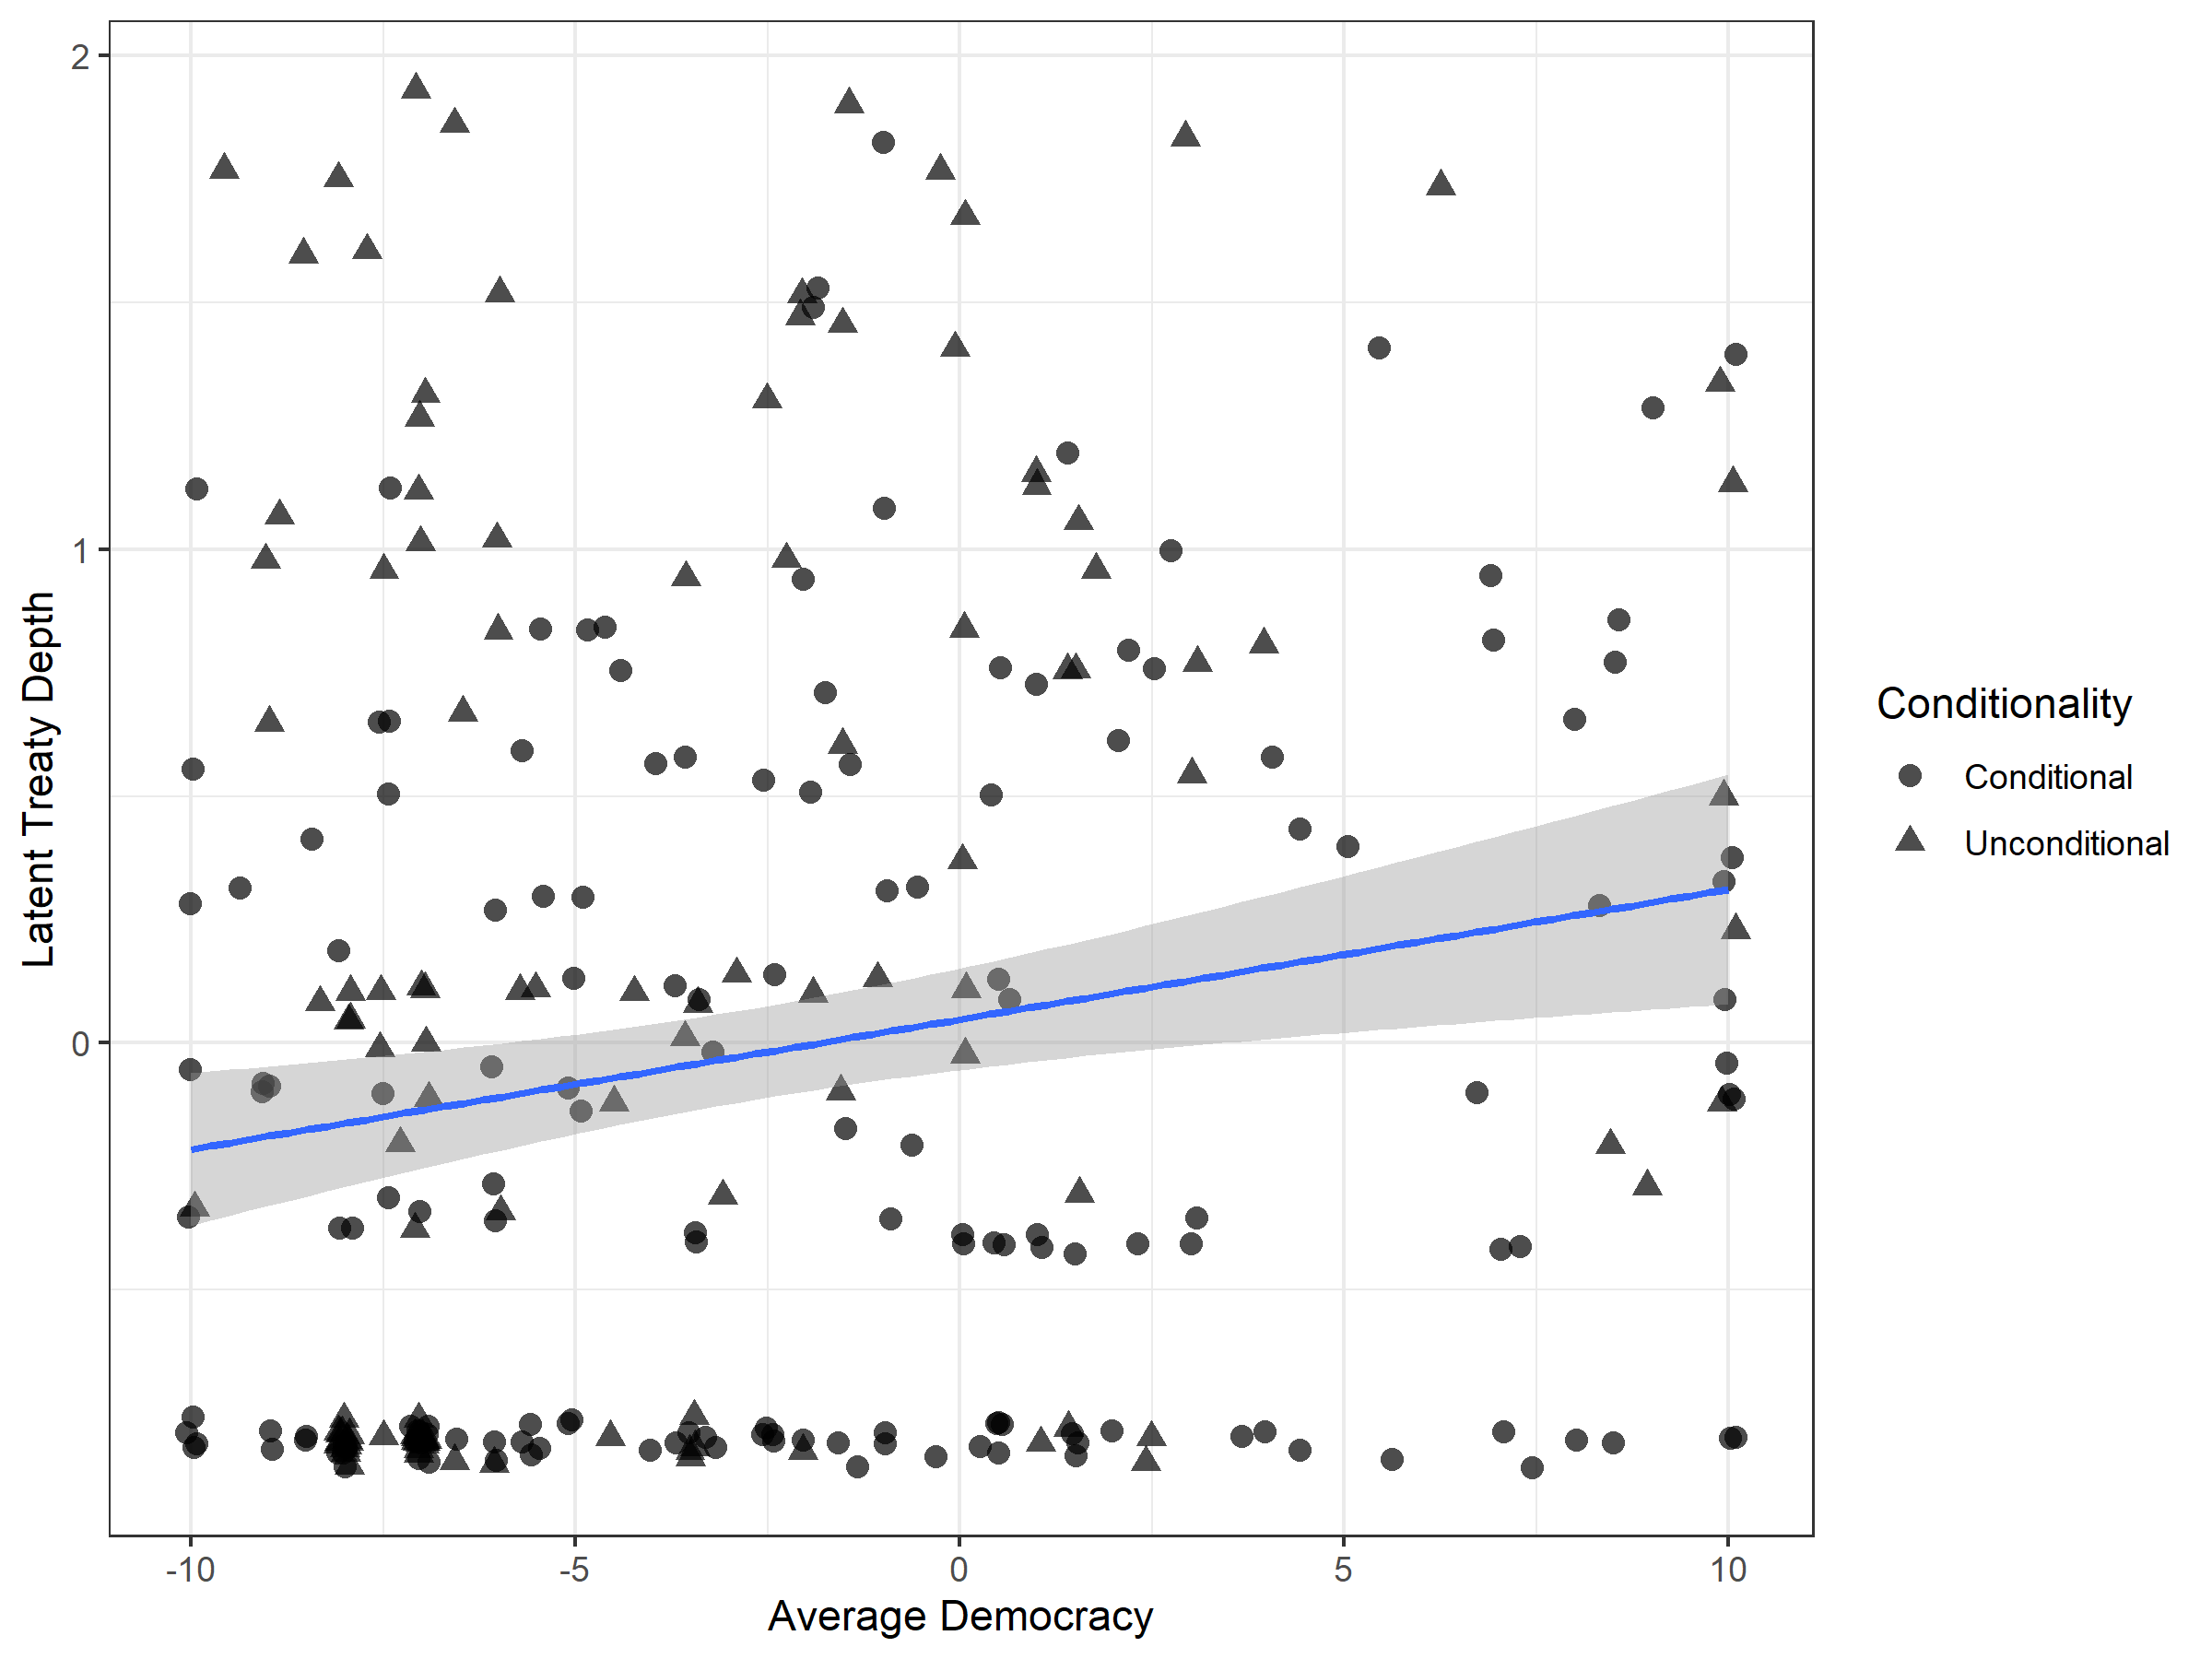
\includegraphics[width=0.95\textwidth]{../figures/democ-combo.png}
\caption{Presence of unconditional military support and depth in alliances from 1816 to 2016. This scatter plot shows mean latent treaty depth on the y-axis and the average polity score of founding alliance members on the x-axis. Triangular points mark treaties with unconditional military support, and the smoothed line trend line is fitted with linear regression. }
\label{fig:democ-combo}
\end{figure}


I now report the results of the joint analysis of depth and unconditional military support. 
\autoref{fig:results-democ} plots the estimated effect of democracy on the two outcomes. 
The predicted effects of democracy on unconditional military support match the two Hypotheses. 
As this figure shows, average democracy impacts both depth and unconditional military support in a very linear fashion. 


\begin{figure}[hbtp]
\centering
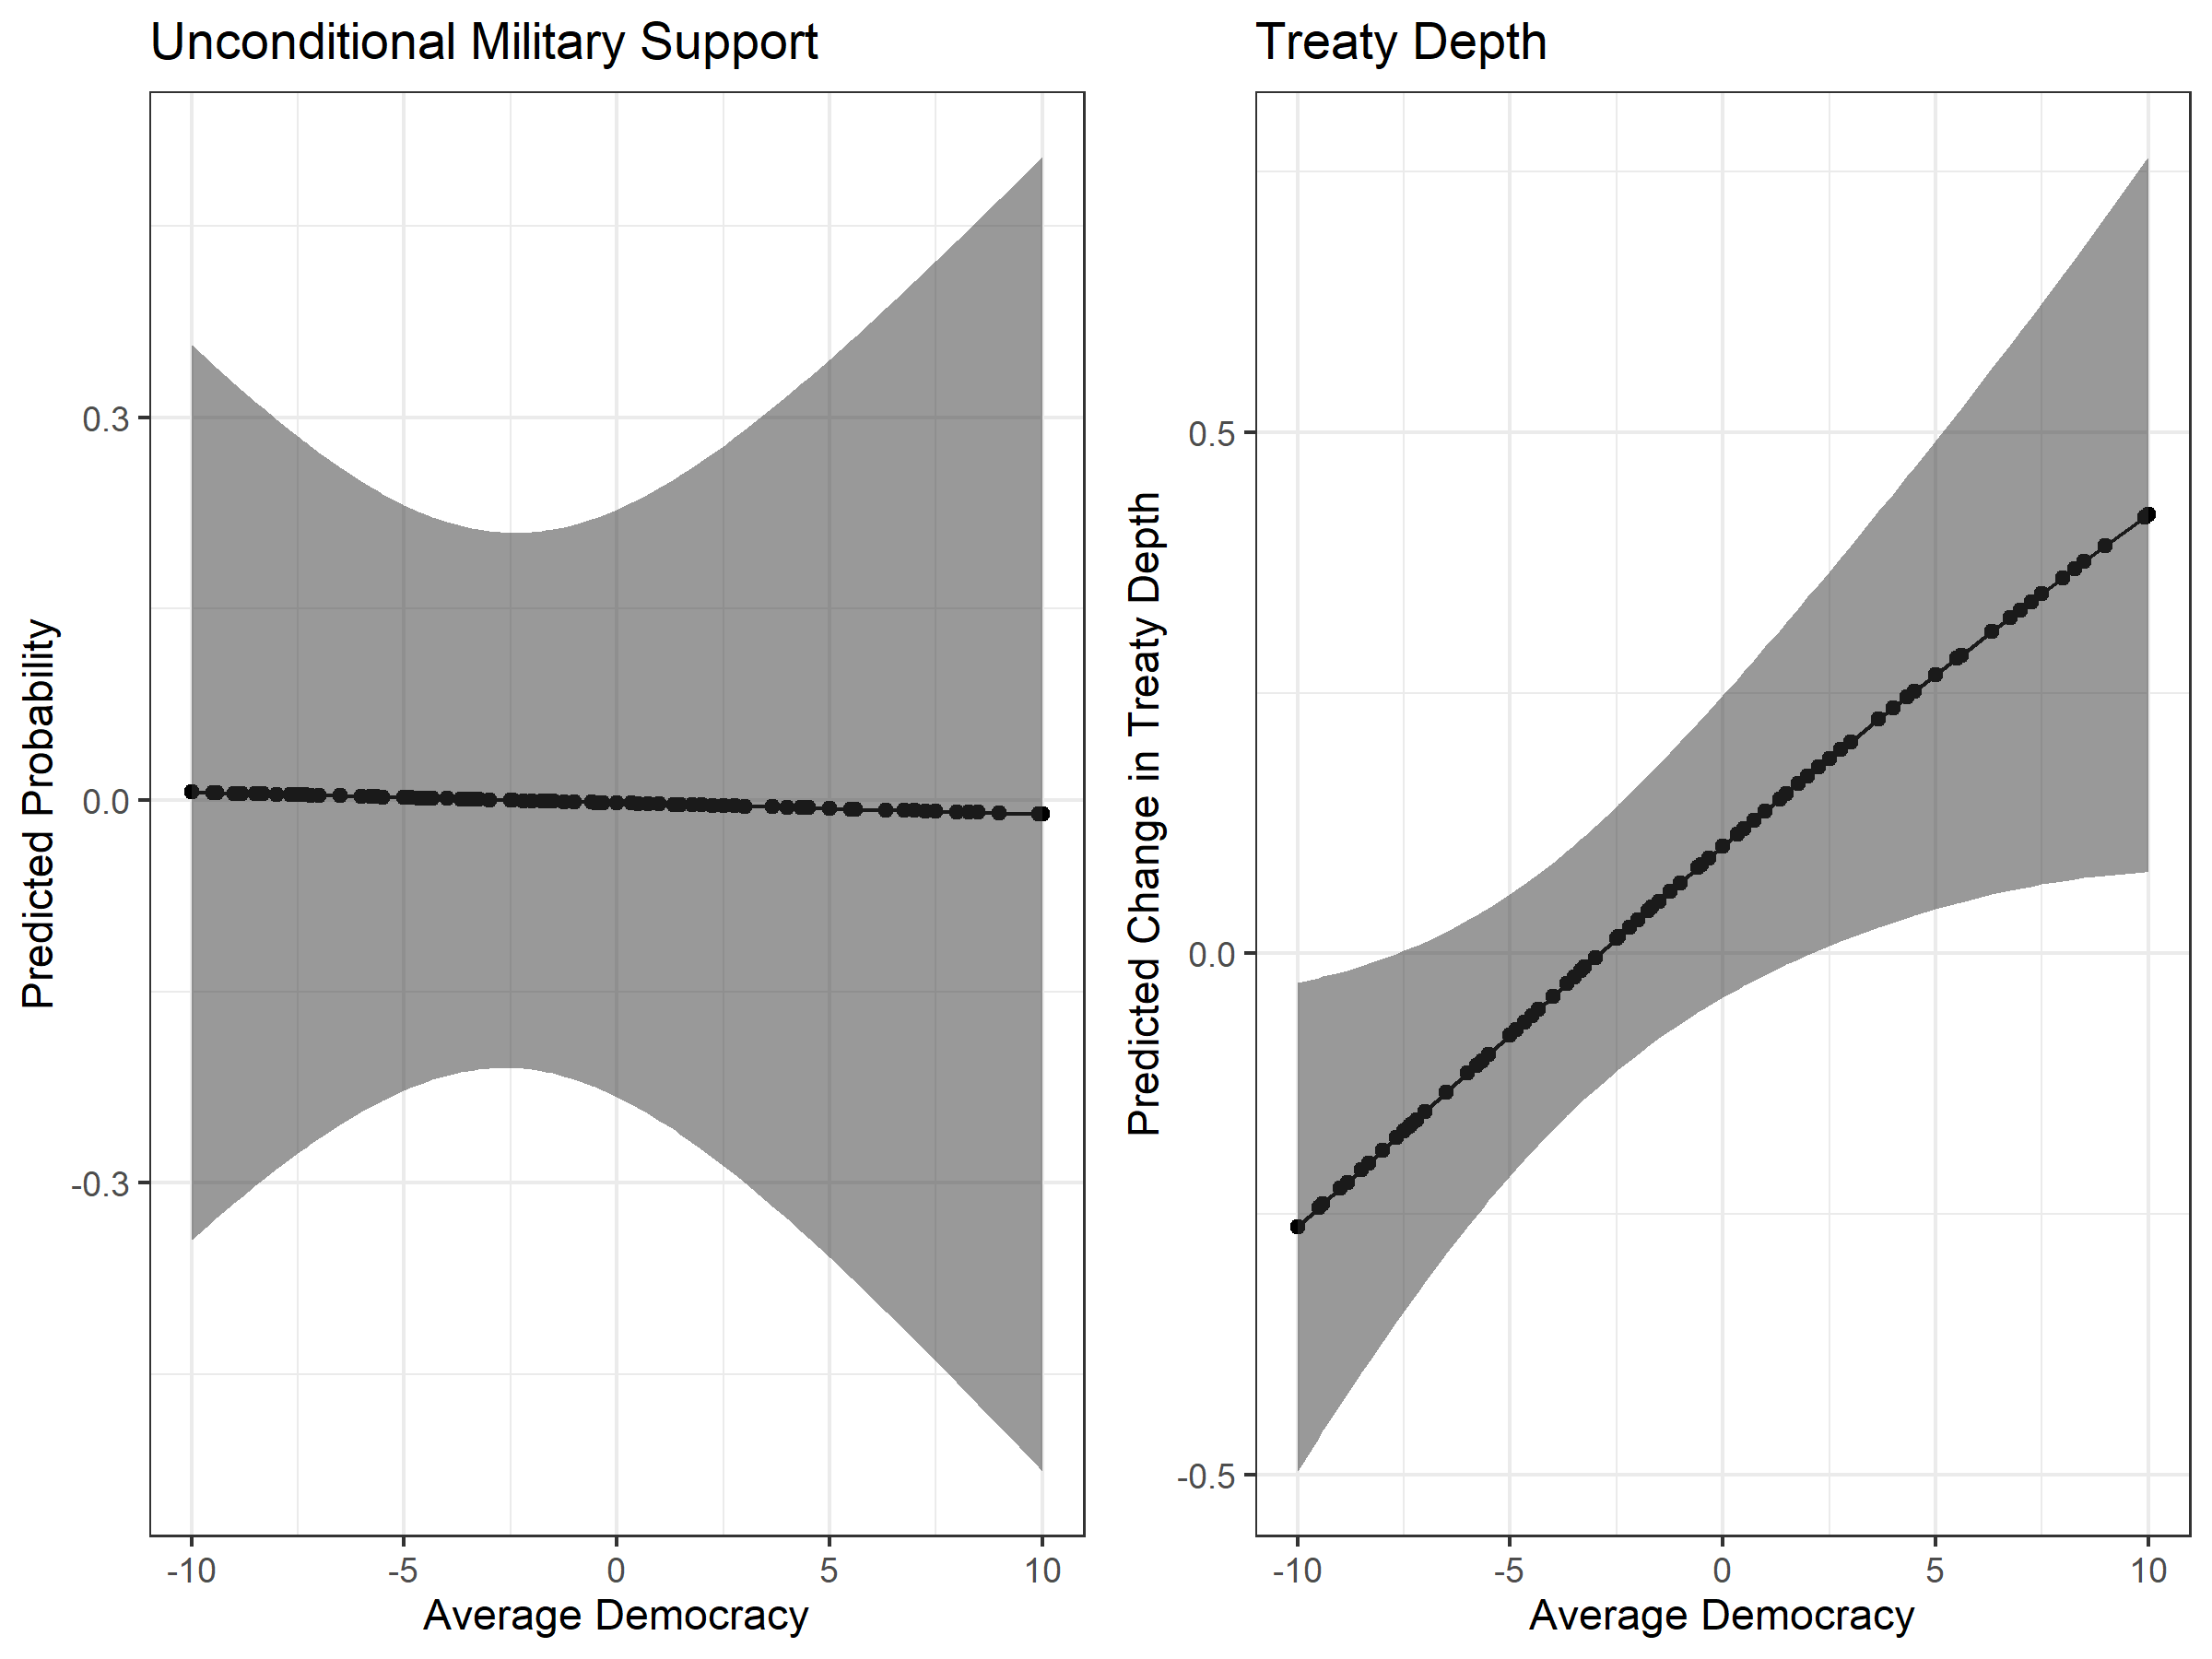
\includegraphics[width=0.95\textwidth]{../figures/results-democ.png}
\caption{Predicted probabilities of unconditional military support and predicted changes in treaty depth across the range of alliance democracy. The line marks predicted values, and the shaded areas encapsulate the standard errors. Points mark observed values of average democracy.}
\label{fig:results-democ}
\end{figure}


The left-hand plot of \autoref{fig:results-democ} shows the association between the average democracy of alliance members and the predicted probability of unconditional military support. 
Highly autocratic alliance membership at the time of alliance formation increases the probability of unconditional military support. 
Alliances with more democratic membership are less likely to offer unconditional military support. 
This finding matches existing results about democracy and conditional commitments \citep{Mattes2012, Chibaetal2015}.


The right-hand plot of \autoref{fig:results-democ} shows that greater democracy at the time of alliance formation increases treaty depth. 
Substantial democracy in an alliance is associated with greater treaty depth. 
Autocracies form shallower alliances, on the other hand. 
This trend of greater depth as the democracy of alliance members rises matches the treaty depth hypothesis. 


There are some other interesting inferences in the control variables, which I present in two tables. 
First, I tabulate the results of the model of unconditional military support in \autoref{tab:uncond-res}.
Depth is positively correlated with the likelihood of unconditional military support.
I also find that asymmetric capability in a treaty and more alliance members decrease the likelihood of unconditional military support. 

\begin{table}[ht]
\centering
\begin{tabular}{rrrrr}
  \hline
 & Estimate & Std. Error & z value & Approx. p-value. \\ 
  \hline 
  Economic Issue Linkage & 0.04 & 0.19 & 0.19 & 0.85 \\ 
  Mean Latent Depth & 4.37 & 0.31 & 14.16 & 0.00 \\ 
  Foreign Policy Concessions & 0.04 & 0.10 & 0.41 & 0.68 \\ 
  Number of Members & -0.04 & 0.02 & -2.82 & 0.00 \\ 
  Wartime Alliance & -0.00 & 0.37 & -0.01 & 0.99 \\ 
  Asymmetric Obligations & -0.12 & 0.21 & -0.57 & 0.57 \\ 
  Asymmetric Capability & -0.43 & 0.20 & -2.17 & 0.03 \\ 
  Foreign Policy Disagreement & -0.00 & 0.31 & -0.00 & 1.00 \\ 
  (Intercept) & -1.25 & 0.31 & -3.98 & 0.00 \\
   \hline
\end{tabular}
\caption{Results from binomial model with a probit link function that predicts the presence of unconditional military support in offensive and defensive alliances from 1816 to 2007.}
\label{tab:uncond-res}
\end{table}



There are also some notable patterns among the other variables in \autoref{tab:depth-res}. 
Unconditional military support is positively correlated with depth, as we would expect from \autoref{tab:uncond-res}. 
Asymmetric capability and the size of the alliance also increase depth. 


\begin{table}[ht]
\centering
\begin{tabular}{rrrrr}
  \hline
 & Estimate & Std. Error & z value & Approx. p-value \\ 
  \hline 
  Economic Issue Linkage & 0.01 & 0.16 & 0.06 & 0.95 \\ 
  Unconditional Support & 0.71 & 0.09 & 8.06 & 0.00 \\ 
  Foreign Policy Concessions & -0.09 & 0.08 & -1.08 & 0.28 \\ 
  Number of Members & 0.02 & 0.01 & 1.70 & 0.09 \\ 
  Wartime Alliance & -0.08 & 0.18 & -0.42 & 0.67 \\ 
  Asymmetric Obligations & 0.19 & 0.17 & 1.11 & 0.27 \\ 
  Asymmetric Capability & 0.31 & 0.14 & 2.19 & 0.03 \\ 
  Foreign Policy Disagreement & 0.24 & 0.23 & 1.05 & 0.30 \\ 
  (Intercept) & -1.29 & 0.22 & -5.93 & 0.00 \\
   \hline
\end{tabular}
\caption{Results from the Beta regression of rescaled treaty depth in offensive and defensive alliances from 1816 to 2007. Smoothed terms for mean threat and start year are not included.}
\label{tab:depth-res}
\end{table}


Based on the coefficients in the model, depth and unconditional military support are positively correlated. 
The errors of the data-generating processes for these two variables are negatively correlated, however. 
Kendall's $\tau$ measures the correlation between the error terms, and it has a mean of -0.956, while the (-0.98,-0.902).
Positive errors in one process are likely to have negative values in the other. 

 
In a separate model, I consider how measurement uncertainty shapes inferences about the connection between non-major power alliances and treaty depth. 
The credible intervals in the bottom panel of \autoref{fig:loadings-measure} show, the latent measure of treaty depth has some uncertainty. 
This is a reasonable approximation of alliance politics, because alliance treaty depth is not observed with certainty. 
There are perceptible differences in treaty depth, especially once states add substantial depth to the treaty. 
Even so, the results from the analysis of mean treaty depth or deep alliance dummy variable may overstate the effect of non-major power membership. 


To address the issue of uncertainty over treaty depth, I fit a modification of the joint model. 
First, I created 1,000 datasets, one for each draw of the posterior distribution of the latent measure.
Then I fit the model of mean treaty depth to 500 randomly sampled datasets from those 1,000 to facilitate computation. 
For models of depth with uncertainty, I use BRMS \citep{Buerkner2017}. 
BRMS is an interface to STAN, a probabilistic programming language for Bayesian estimation \citep{Carpenteretal2016}. 
Joint Bayesian estimation has the flexibility to incorporate the logistic and beta models and can be easily extended to account for uncertainty in the depth measure. 
It does not allow correlated errors, however.
This produces 500 separate models, which I combine into a single model. 
With fully Bayesian inference, I can aggregate the posterior draws in a single posterior that accounts for uncertainty in the treaty depth measure.\footnote{Standard convergence diagnostics indicate convergence in each of the submodels. Diagnostics like $\hat{r}$ are less useful for the full posterior, because some of the chains in the submodels do not overlap.}
This approach is analogous to common techniques for analyzing missing data, where multiple imputation generates uncertainty about the missing values \citep{Hollenbachetal2018imp}.
Under these conditions, researchers fit a separate model to each of the imputed datasets and then combine the results. 


% Expand on these results later 
After accounting for uncertainty over treaty depth, I find a similar pattern. 
Allied democracy increases treaty depth, but decreases the probability of unconditional military support. 
These aggregate patterns give some sense of the theoretical process. 
To corroborate my theoretical claim that democracies substitute depth for unconditional support, I now offer a brief case study. 


\subsection{Case Study}


The case study examines the alliance negotiation process in two treaties. 
By tracing the process of alliance negotiations, I show how allied democracy shapes unconditional military support and treaty depth, and that states traded off between depth and scope. 
I explore the process behind a 1966 alliance between Mongolia and the USSR (ATOPID 3535) and a 1976 pact between Spain and the United States (ATOPID 3750). 


I selected these cases using matching software, following the recommendations of \citet{Nielsen2016}. 
Case selection is a crucial part of process tracing \citep{SeawrightGerring2008}, and matching cases makes selection more transparent and replicable. 
Moreover, matching cases on observed confounders allows researchers to contend with alternative explanations that are not addressed by matching \citep{Nielsen2016}. 


Because I am interested in the causal mechanism behind high treaty depth, I matched on key control variables in the analysis and used the average democracy variable as the treatment. 
I did not include unconditional military support as a matching variable, because it is part of the process. 
The specific matching pair I chose did not have the minimum Mahalanobis distance, but it had high outcome variance and differences in the key independent variable.\footnote{The main sources of imbalance are a slight difference in foreign policy similarity and a 10-year difference in the start year of the treaty.} 


\section{Discussion}


% main evidence for an indirect effect
The findings from the statistical model (and maybe the case study) are consistent with my claim that democracies substitute treaty depth for conditions on military support. 
Although democracies tend to provide conditional military support, they use depth as an alternative means of establishing reliability. 

 
My findings suggest that the conventional wisdom democracies make limited alliance commitments is partially correct.
Democracies do offer limited support, at least in the scope of their treaties. 
But democracies are more prone to increase the depth of their alliances. 
Alliances with democratic membership are limited in one dimension, but deep in another. 


% Therefore, sources of alliance credibility are rather entangled
My findings show how different aspects of alliance treaty design are related. 
\citet{BensonClinton2016} use measurement models to show this in a descriptive fashion, but my findings give a sense of the process behind different combinations of depth and conditions on military support. 
Previous research on the causes of alliance treaty design \citep{Benson2012, Mattes2012, Chibaetal2015} focused on particular characteristics and treated them as independent. 
My results suggest that this approach can be informative, but it is incomplete. 


Different sources of alliance treaty credibility are thoroughly entangled. 
Depth and unconditional military support are closely related because democracies substitute between these sources of credibility, but autocracies use them as complements. 
This has important implications for scholarship. 


\section{Conclusion}


Understanding the sources of alliance treaty depth helps clarify the how to model the way depth affects other outcomes, such as military spending by alliance participants. 
Adjusting for regime type is a simple . 
Moreover, given the sequence of alliance treaty negotiations, neither alliance treaty member characteristics or conditions on military support are post-treatment variables for treaty depth. 


The key implication for scholarship is that alliance treaty design is the result of a series of correlated decisions. 
Rather than address each part of treaty design piecemeal, scholars should think about connections between the core aspects of treaty design. 
For example, future work might examine the connections between conditions on military support, treaty depth, and issue linkages.  
Debating what promises to include among these core obligations will be a crucial next step. 
Any discussion of alliance treaty design must also situate these decisions in the process of treaty negotiations.
As such, my findings support calls to correct the comparative neglect of negotiations in existing scholarship \citep{Poast2019a}. 


Last, alliances are an international institution, so some of the lessons from this work may apply to other institutions. 
There is an extensive literature on the design on international institutions \citep{DownesRocke1995, MartinSimmons1998, Koremenosetal2001, Koremenos2005, Thompson2010}.
Debates about the trade off between breadth and depth \citep{Downsetal1998, Gilligan2004} reflect correlated design decisions given potential institutional membership. 
Still, this literature could adopt a similar emphasis on the sequence of negotiations to clarify how different aspects of institutional design are related. 


In conclusion, democratic alliance membership is a source of treaty depth. 
Democracies often substitute treaty depth for unconditional military support. 
This shows how different sources of reliability shapes alliance treaty negotiations. 



\singlespace
 
\bibliography{../../../MasterBibliography} 





\end{document}